\chapter{\texorpdfstring{Algebras of $\PaB$}{Algebras of PaB}}
\lhead{\emph{algebras of $\PaB$}}
\section{Braided Monoidal Categories}
\begin{definition}[monoidal category]
	A category $\sC$ with a bifunctor $-\otimes-:\sC\times\sC\to\sC$ (the monoidal, or tensor product), unit object $\mathbf{1}$, and natural isomorphisms
	\begin{align}
		&a:(-\otimes-)\otimes-\Rightarrow-\otimes(-\otimes-)\\
		&l:\mathbf{1}\otimes-\Ra\id_\sC & r:-\otimes\mathbf{1}\Ra\id_{sC}
	\end{align}
	 respectively called the associator, left unitor, right unitor, is \emph{monoidal} if when we write $\otimes$ to act componentwise on natural transformations,
	\begin{enumerate}
	\item the triangle identity is satisfied, i.e. $r\otimes\id_\sC=(\id_\sC\otimes l)\circ a$
	\item the pentagon identity holds, i.e. for all $w,x,y,z\in\Obj(\sC)$, the following diagram commutes
	

\tikzset{every picture/.style={line width=0.75pt}} %set default line width to 0.75pt        
\[
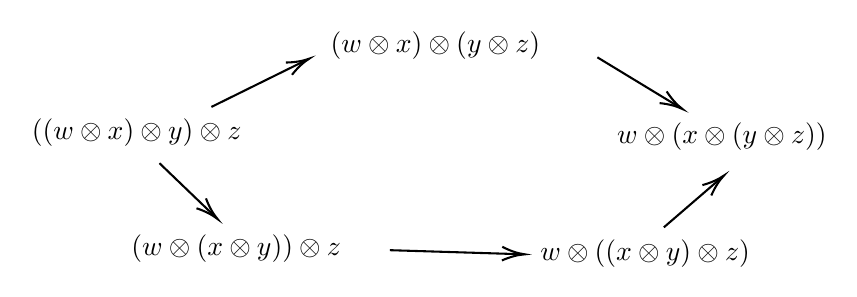
\begin{tikzpicture}[x=0.75pt,y=0.75pt,yscale=-1,xscale=1]
%uncomment if require: \path (0,497); %set diagram left start at 0, and has height of 497

%Straight Lines [id:da8091689343428804] 
\draw    (162,295.1) -- (207.41,272.69) ;
\draw [shift={(209.2,271.8)}, rotate = 153.73] [color={rgb, 255:red, 0; green, 0; blue, 0 }  ][line width=0.75]    (10.93,-3.29) .. controls (6.95,-1.4) and (3.31,-0.3) .. (0,0) .. controls (3.31,0.3) and (6.95,1.4) .. (10.93,3.29)   ;
%Straight Lines [id:da5599598183630712] 
\draw    (348,271.2) -- (387.29,295.06) ;
\draw [shift={(389,296.1)}, rotate = 211.27] [color={rgb, 255:red, 0; green, 0; blue, 0 }  ][line width=0.75]    (10.93,-3.29) .. controls (6.95,-1.4) and (3.31,-0.3) .. (0,0) .. controls (3.31,0.3) and (6.95,1.4) .. (10.93,3.29)   ;
%Straight Lines [id:da8391035848401762] 
\draw    (137,322.2) -- (163.56,347.71) ;
\draw [shift={(165,349.1)}, rotate = 223.85] [color={rgb, 255:red, 0; green, 0; blue, 0 }  ][line width=0.75]    (10.93,-3.29) .. controls (6.95,-1.4) and (3.31,-0.3) .. (0,0) .. controls (3.31,0.3) and (6.95,1.4) .. (10.93,3.29)   ;
%Straight Lines [id:da28460978615375354] 
\draw    (248,364.1) -- (311,366.04) ;
\draw [shift={(313,366.1)}, rotate = 181.76] [color={rgb, 255:red, 0; green, 0; blue, 0 }  ][line width=0.75]    (10.93,-3.29) .. controls (6.95,-1.4) and (3.31,-0.3) .. (0,0) .. controls (3.31,0.3) and (6.95,1.4) .. (10.93,3.29)   ;
%Straight Lines [id:da9551788148488187] 
\draw    (380,353.1) -- (407.49,329.41) ;
\draw [shift={(409,328.1)}, rotate = 139.24] [color={rgb, 255:red, 0; green, 0; blue, 0 }  ][line width=0.75]    (10.93,-3.29) .. controls (6.95,-1.4) and (3.31,-0.3) .. (0,0) .. controls (3.31,0.3) and (6.95,1.4) .. (10.93,3.29)   ;

% Text Node
\draw (74,299.4) node [anchor=north west][inner sep=0.75pt]    {$(( w\otimes x) \otimes y) \otimes z$};
% Text Node
\draw (218,257.4) node [anchor=north west][inner sep=0.75pt]    {$( w\otimes x) \otimes ( y\otimes z)$};
% Text Node
\draw (356,301.4) node [anchor=north west][inner sep=0.75pt]    {$w\otimes ( x\otimes ( y\otimes z))$};
% Text Node
\draw (122,355.4) node [anchor=north west][inner sep=0.75pt]    {$( w\otimes ( x\otimes y)) \otimes z$};
% Text Node
\draw (319,357.4) node [anchor=north west][inner sep=0.75pt]    {$w\otimes (( x\otimes y) \otimes z)$};


\end{tikzpicture}
\]
	or as natural transformations, $a\circ a=(\id_\sC\otimes a)\circ a\circ(a\otimes\id_\sC)$
	\end{enumerate}
\end{definition}

A monoidal category is \emph{strict} if the components of the associator and unitors are identity morphisms.
\begin{definition}[braided monoidal category] \label{braidedMonoidalCategory}
	If $(\sC,\otimes,\mathbf{1},a,l,r)$ is a monoidal category with a natural isomorphism $b_{x,y}:x\otimes y\to y\otimes x$, then it is \emph{braided} if it satisfies the hexagon identities, i.e. the following diagrams commute
	\[
\begin{tikzcd}
	% https://tikzcd.yichuanshen.de/#N4Igdg9gJgpgziAXAbVABwnAlgFyxMJZABgBpiBdUkANwEMAbAVxiRAAoAPAHW4jwC28AAQBPAJS9+WIXGEAvEAF9S6TLnyEUARnJVajFmx59B8dqKlm588ctUgM2PASIAmPdXrNWiDpdMZEVsrILlOezVnTSIybX1vIz8LUNlhTklAtMUVKI1XHVJ4r0NfEADpWS5U4Ltcx3UXLWQPYoMfNgrrdnka8Lr9GCgAc3giUAAzACcIASQyEBwIJABmEo6-ACNea14sKAB9XjgAYRBqBjpNmAYABUaYvwYYCZxIkGnZ+eolpF12pIgOjnECXa53B4FUEvN71T5zRD-X6IDwAsqbEFgm73aJQ56vd7wpCo5EAVnWgOBFyu2MhWmhBLhMwRa0Wy0QABYKWUqaCaRDcfT8bCHETOT92eS+eCcfkhTCQYkyntDscTn1hBilBQlEA
(x\otimes y)\otimes z \arrow[d, "b\times\id_\sC"] \arrow[r, "a"] & x\otimes(y\otimes z) \arrow[r, "b"]                & (y\otimes z)\otimes x \arrow[d, "a"] \\
(y\otimes x)\otimes z \arrow[r, "a"]                             & y\otimes(x\otimes z) \arrow[r, "\id_\sC\otimes b"] & y\otimes(z\otimes x)                
\end{tikzcd}
	\]
	\[\begin{tikzcd}
		% https://tikzcd.yichuanshen.de/#N4Igdg9gJgpgziAXAbVABwnAlgFyxMJZABgBpiBdUkANwEMAbAVxiRAA8AdTiPAW3gAKAJ7deWAXAAEALwCUIAL6l0mXPkIoAjOSq1GLNoK49+8KcLliz0mUpUgM2PASIAmXdXrNWiEDOsJIRNxSQsFZVVnDXdSLT1vQz9BANMg6XYrNLDheyj1VxQyeK8DXw5AyRTK80s8xzUXTWQdEv0fIxCbWSzQ2qU9GCgAc3giUAAzACcIPiQyEBwIJB12pJA6AD1gAFotRXrp2ZXqJaQPNfKAI0OZucQLs8QAZlKOvy3d-dvjxAWngAsb3W3CwUAA+tw4ABhGrSG6REBHe5AxbLRAAVmB5U+ewOiORSCxaKQr0ubCucNBEKh0IGiiAA
x\otimes(y\otimes z) \arrow[r, "a^{-1}"] \arrow[d, "\id_\sC\otimes b"] & (x\otimes y)\otimes z \arrow[r, "b"]               & z\otimes(x\otimes y) \arrow[d, "a^{-1}"] \\
x\otimes(z\otimes y) \arrow[r, "a^{-1}"]                               & (x\otimes z)\otimes y \arrow[r, "b\otimes\id_\sC"] & (z\otimes x)\otimes y                   
\end{tikzcd}\]
\end{definition}

We will now build up to Mac Lane's Coherence Theorem
\begin{definition}[monoidal functor, or strong monoidal functor at nLab]
	Suppose $(\sC,\otimes,\mathbf{1},a,l,r)$, and $(\sC',\otimes',\mathbf{1}',a',l',r')$, are monoidal categories, then a monoidal functor consists of a functor $F:\sC\to\sC'$ such that $\mathbf{1'}\cong F(\mathbf{1})$, and a natural isomorphism $m:F(-)\otimes F(-)\to F(-\otimes-)$ such that the following diagram commutes
	\[\begin{tikzcd}
		% https://tikzcd.yichuanshen.de/#N4Igdg9gJgpgziAXAbVABwnAlgFyxMJZABgBpiBdUkANwEMAbAVxiRAAoAxdgDQEoAOgIh4AtvAAE3AJp9BwsZO4AtPiAC+pdJlz5CKAIzkqtRizbceQkVnFwJs64vsq1m7djwEiAJmPV6ZlZEEG5eJ1tJRwVI+1UNLRAMTz1fUgMTQPMQywi7dmk8yVU3ROTdbxQyDICzYNDeeRt8mSbnKXYShI8K-WQjGtMgi0ailwKxiXj1ExgoAHN4IlAAMwAnCFEkMhAcCCQjIeyQUTGhLCgAfSE4AGFukHXNg+o9pD8j+q33R42txA+b0QAGZasMcuw6KVVn9tq99ogACxg450ADkDye-2RuwRAFYUfVzlcbrdJt9ElikATcUhQZ82N8KOogA
(F(X)\otimes F(Y))\otimes F(Z) \arrow[r, "m\otimes\id_\sC"] \arrow[d, "a'"] & F(X\otimes Y)\otimes F(Z) \arrow[r, "m"] & F((X\otimes Y)\otimes Z) \arrow[d, "F(a)"] \\
F(X)\otimes(F(Y)\otimes F(Z)) \arrow[r, "\id_\sC\otimes m"]                 & F(X)\otimes F(Y\otimes Z) \arrow[r, "m"] & F(X\otimes(Y\otimes Z))                   
\end{tikzcd}\]
\end{definition}
A monoidal functor that happens to be an equivalence of categories is called an \emph{equivalence of monoidal categories}.
\begin{theorem}[Mac Lane's Strictness Theorem]
	For any monoidal category $(\sC,\otimes,\mathbf{1},a,l,r)$, there exists a \emph{strict} monoidal category $(\sC',\otimes',\mathbf{1}',a',l',r')$ and an equivalence of monoidal categories $L:\sC\to\sC'$.
\end{theorem}
\begin{proof}
	see \cite{Etingof} from the 2009 lecture notes to "Topics in Lie Theory".
	% Let $\sC'$ be pairs $(F,c)$ where $F$ is an endofunctor of $\sC$, and $c:F(-)\otimes\id_\sC\to F(-\otimes\id_\sC)$ is a natural isomorphism. Then $\sC'$ is strict, and we can construct an equivalence of monoidal categories $L:\sC\to\sC'$ by left multiplication:
	% \begin{enumerate}
	% 	\item For all $X\in\Obj(\sC)$, $L(X)\defeq X\otimes-$.
	% 	\item For morphisms $f$ in $\sC$, $L(f)\defeq f\otimes-$.
	% \end{enumerate}
\end{proof}
The next theorem is a corollary of Mac Lane's Strictness Theorem.
\begin{theorem}[Mac Lane's Coherence Theorem]
	Suppose $P$ and $P'$ are parenthesizations of $X_1\otimes\cdots\otimes X_n$ with arbitrary insertions of $\mathbf{1}$, and $f,g:P\to P'$ are isomorphisms built by composing associator and unitor components, then $f=g$.
\end{theorem}
\begin{proof}
	see \cite{Etingof_2009}
\end{proof}
\section{\texorpdfstring{The Operad $\PaB$ of Parenthesized Braids}{The Operad PaB of Parenthesized Braids}}
\begin{definition}[operad]
	An operad $P$ in a monoidal category $(\sC,\otimes,\mathbf{1},a,l,r)$ is a collection of objects $\left\{ P(n) \right\}_n$, each object $P(n)$ has a right $S_n$-action ($S_n$ being the $n$th symmetric group), and operadic composition $\circ_i:P(m)\otimes P(n)\to P(m+n-1)$ such that
\end{definition}